\documentclass[12pt]{article}
\usepackage[margin=1in]{geometry}

% Start of preamble
%==========================================================================================%
% Required to support mathematical unicode
\usepackage[warnunknown, fasterrors, mathletters]{ucs}
\usepackage[utf8x]{inputenc}

\usepackage[dvipsnames,table,xcdraw]{xcolor}
\usepackage{hyperref} 
\hypersetup{
colorlinks=true,
linkcolor=blue,
filecolor=magenta,
urlcolor=cyan,
pdfpagemode=FullScreen
}

% Standard mathematical typesetting packages
\usepackage{amsmath,amssymb,amscd,amsthm,amsxtra, pxfonts}
\usepackage{mathtools,mathrsfs,dsfont,xparse}

% Symbol and utility packages
\usepackage{cancel, textcomp}
\usepackage[mathscr]{euscript}
\usepackage[nointegrals]{wasysym}
\usepackage{apacite}

% Extras
\usepackage{physics}  
\usepackage{tikz-cd} 
\usepackage{microtype}
\usepackage{enumitem}
\usepackage{titling}
\usepackage{graphicx}

% Fancy theorems due to @intuitively on discord
\usepackage{mdframed}
\newmdtheoremenv[
backgroundcolor=NavyBlue!30,
linewidth=2pt,
linecolor=NavyBlue,
topline=false,
bottomline=false,
rightline=false,
innertopmargin=10pt,
innerbottommargin=10pt,
innerrightmargin=10pt,
innerleftmargin=10pt,
skipabove=\baselineskip,
skipbelow=\baselineskip
]{mytheorem}{Theorem}

\newenvironment{theorem}{\begin{mytheorem}}{\end{mytheorem}}

\newtheorem{corollary}{Corollary}
\newtheorem{lemma}{Lemma}

\newtheoremstyle{definitionstyle}
{\topsep}%
{\topsep}%
{}%
{}%
{\bfseries}%
{.}%
{.5em}%
{}%
\theoremstyle{definitionstyle}
\newmdtheoremenv[
backgroundcolor=Violet!30,
linewidth=2pt,
linecolor=Violet,
topline=false,
bottomline=false,
rightline=false,
innertopmargin=10pt,
innerbottommargin=10pt,
innerrightmargin=10pt,
innerleftmargin=10pt,
skipabove=\baselineskip,
skipbelow=\baselineskip,
]{mydef}{Definition}
\newenvironment{definition}{\begin{mydef}}{\end{mydef}}

\newtheorem*{remark}{Remark}

\newtheorem*{example}{Example}

% Common shortcuts
\def\mbb#1{\mathbb{#1}}
\def\mfk#1{\mathfrak{#1}}

\def\bN{\mbb{N}}
\def \C{\mbb{C}}
\def \R{\mbb{R}}
\def\bQ{\mbb{Q}}
\def\bZ{\mbb{Z}}
\def \cph{\varphi}
\renewcommand{\th}{\theta}
\def \ve{\varepsilon}
\newcommand{\mg}[1]{\| #1 \|}

% Often helpful macros
\newcommand{\floor}[1]{\left\lfloor#1\right\rfloor}
\newcommand{\ceil}[1]{\left\lceil#1\right\rceil}
\renewcommand{\qed}{\hfill\qedsymbol}
\renewcommand{\P}{\mathbb P\qty}
\newcommand{\E}{\mathbb{E}\qty}
\newcommand{\Cov}{\mathrm{Cov}\qty}
\newcommand{\Var}{\mathrm{Var}\qty}

% Sets
\usepackage{braket}

\graphicspath{{/}}
\usepackage{float}

\newcommand{\SET}[1]{\Set{\mskip-\medmuskip #1 \mskip-\medmuskip}}

% End of preamble
%==========================================================================================%

% Start of commands specific to this file
%==========================================================================================%

%==========================================================================================%
% End of commands specific to this file

\title{CSE 446 HW2}
\date{\today}
\author{Rohan Mukherjee}

\begin{document}
    \maketitle
    \subsection*{A1.}  
    \begin{enumerate}[label=\alph*.]
        \item In the L1 norm, small numbers are punished more than in the L2 norm. For example, in the L2 norm a coordinate of 0.1 translates to an increase in only 0.01, which is almost negligible. But in the L1 norm it still has a lot of weight.
        \item This is true, since we might step past the minimum with too large a step size, and then we will try to step back towards it, but just end up oscillating far from the minimum.
        \item SGD runs much, much faster than GD, bringing the running time from $O(n \cdot d)$ per iteration to only $O(d)$. GD on the other hand is much more stable, not relying on randomness and we don't have to worry about changing the step size in the process.
        \item Logistic regression does not have a closed form solution, while linear regression does.
    \end{enumerate}

    \subsection*{A2.}
    \begin{enumerate}[label=\alph*.]
        \item Since $|ax| = |a||x|$ holds for all $a,x \in \R$, we must have $\sum_{i=1}^n |ax_i| = \sum_{i=1}^n |a||x_i| = |a|\sum_{i=1}^n |x_i|$. Also, $|x| \geq 0$ for every $x \in \R$, so $\sum_{i=1}^n |x_i| \geq 0$. Finally, notice that
        \begin{align*}
            (|a+b|)^2 = (a+b)^2 = a^2+b^2+2ab \leq a^2+b^2+2|a||b| = (|a|+|b|)^2
        \end{align*}
        Since $f(x) = \sqrt{x}$ is increasing, and both the LHS and RHS are positive, taking square roots on both sides shows that $|a+b| \leq |a| + |b|$. Using this repeatedly yields:
        \begin{align*}
            \sum_{i=1}^n |x_i+y_i| \leq \sum_{i=1}^n |x_i| + |y_i| = \sum_{i=1}^n |x_i| + \sum_{i=1}^n |y_i|
        \end{align*}
        \item Consider the vectors $x = (1/4, 0)$ and $y = (0, 1/4)$. Then,
        \begin{align*}
            g(x+y) = \qty(\frac{1}{2} + \frac{1}{2})^2 = 1
        \end{align*}
        while,
        \begin{align*}
            g(x) + g(y) = \frac{1}{4} + \frac{1}{4} = \frac{1}{2}
        \end{align*}
        Which shows that the triangle inequality does not hold.
    \end{enumerate}

    \subsection*{A3.}
    Note that the set of points $\SET{\lambda a + (1-\lambda)b \mid 0 \leq \lambda \leq 1} = \SET{a + \lambda(b-a) \mid 0 \leq \lambda \leq 1}$ is precisely the lien conneting $a$ with $b$. Since in part I, the line connecting the point $b$ with $c$ does not live fully within the set, we see that I is not convex. Similarly, applying the same logic to points a and d in the second picture shows that the II is not convex either.

    \subsection*{A4.}
    The first function I is convex because it is a quadratic function pointing upwards, with always-positive second derivative. The second function is not convex because The secant line between $b$ and $c$ lies below the curve, not above it (Recall that the line $\lambda f(x) + (1-\lambda)f(y)$ for $0 \leq \lambda \leq 1$ is the secant line of $f$ between $x$ and $y$).

    \subsection*{A5.}
    \begin{enumerate}[label=\alph*.]
        \item[(a/b).] Here are my graphs, where $\mathrm{nnz}(w)$ is the number of non-zero elements in $w$:
        \begin{figure}[H]
            \centering
            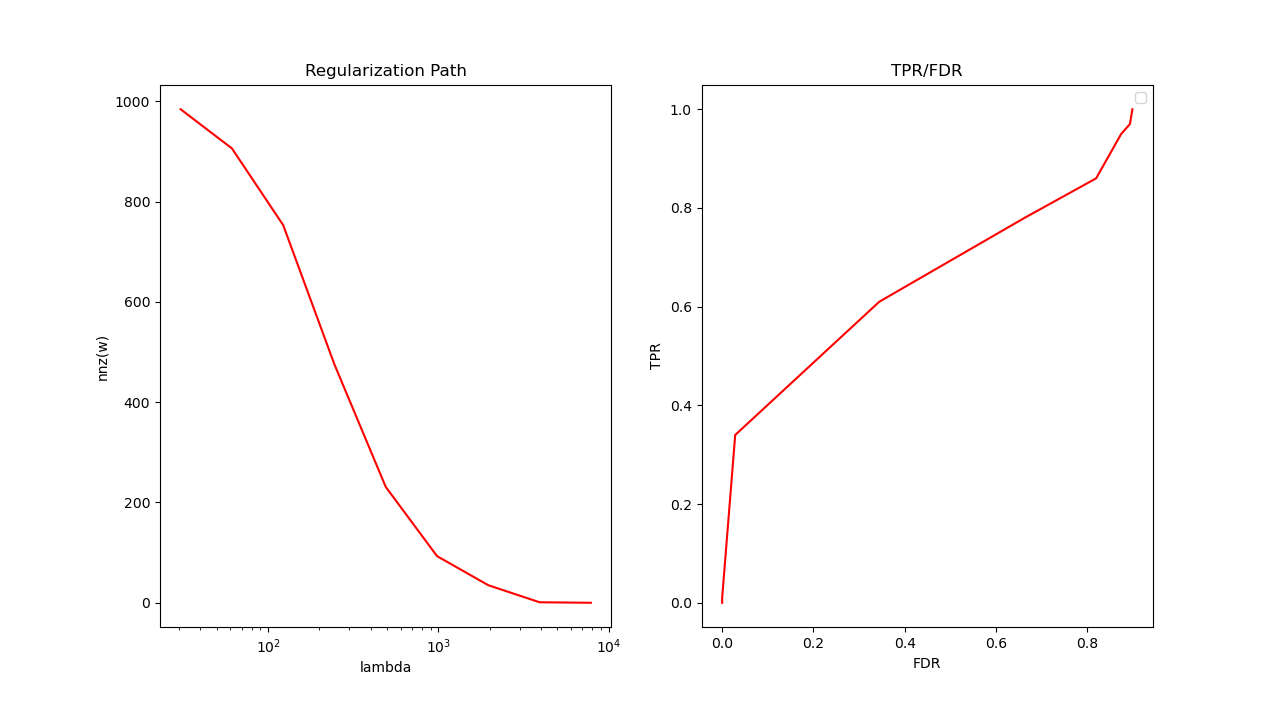
\includegraphics[width=\textwidth]{regpath_fdr_tpr.png}
            \caption{nnz(w) as a function of $\lambda$ and FDR vs TPR}
        \end{figure}

        \item[c.] We can see on the left that increasing $\lambda$ decreases the number of nonzero entries in $w$, as expected. On the right, recall that $\lambda_{max}$ was chosen to have all zero entries, equivalently having a true positive rate of 0. Thus as $\lambda$ shrinks, the true positive rate and the false positive rate both increase. I would guess that the sweet spot is where the FDR is really small and the TPR is reasonably large, equivalently when the slope is really high. This occurs around FDR = 0.05. Thus there is a trade off with $\lambda$--smaller $\lambda$ makes the number of nonzeros much smaller while at the same time making the false positive rate and true positive rate higher.
    \end{enumerate}

    \subsection*{A6.}
    \begin{enumerate}[label=\alph*.]
        \item PCTNotHSGrad, PCTLargHouseOccup, and PCTUsePubTrans
        In a lot of less wealthy communities, the education system is either a lot worse due to little investment, so due to government policies like not having enough tax dollars to invest in schools the graduation rate can be lower. Similarly, wealther communities tend to have less single-family housing, and even some policies that prevent more single family housing, so the percentange of large house occupancy can go down. Finally, the percentage of people using public transportation is entirely dependent on the amount of investment the government has put into public transportation, so that varies a lot depending on policy.

        \item Three features that might be interpreted as reasons for higher levels of violent crime are the PctUnemployed, pctNotHSGrad, and LemasSwornFT. When working at a store is more dangerous less people will want to, making PctUnemployed go up, violent crime in the neighborhood can prevent kids from going to school because they want to stay safe, and finally, police offers are not commiting crimes but are instead are trying to stop them, so show up near crime a lot, so a higher LemasSwornFT could be misinterpreted as a cause of violent crime.
        
        \item The nonzero weights as a function of $\lambda$ can be seen in the following graph:
        \begin{figure}[H]
            \centering
            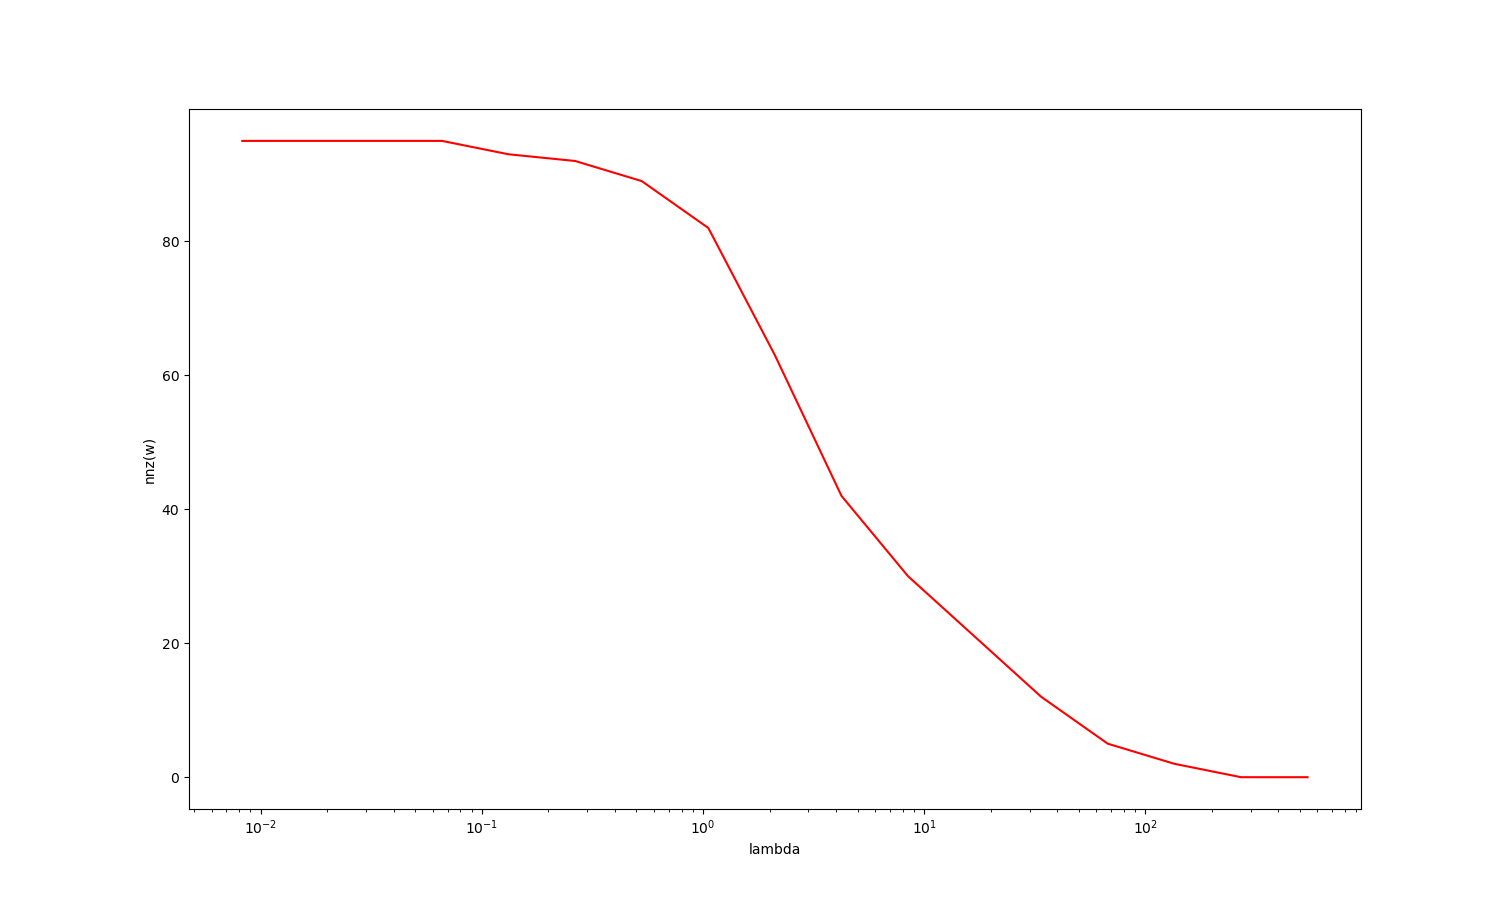
\includegraphics[width=0.8\textwidth]{crime_nonzero_weights.png}
            \caption{Nonzero weights as a function of $\lambda$}
        \end{figure}

        \item The regularization paths for the coefficients of those variables is:
        \begin{figure}[H]
            \centering
            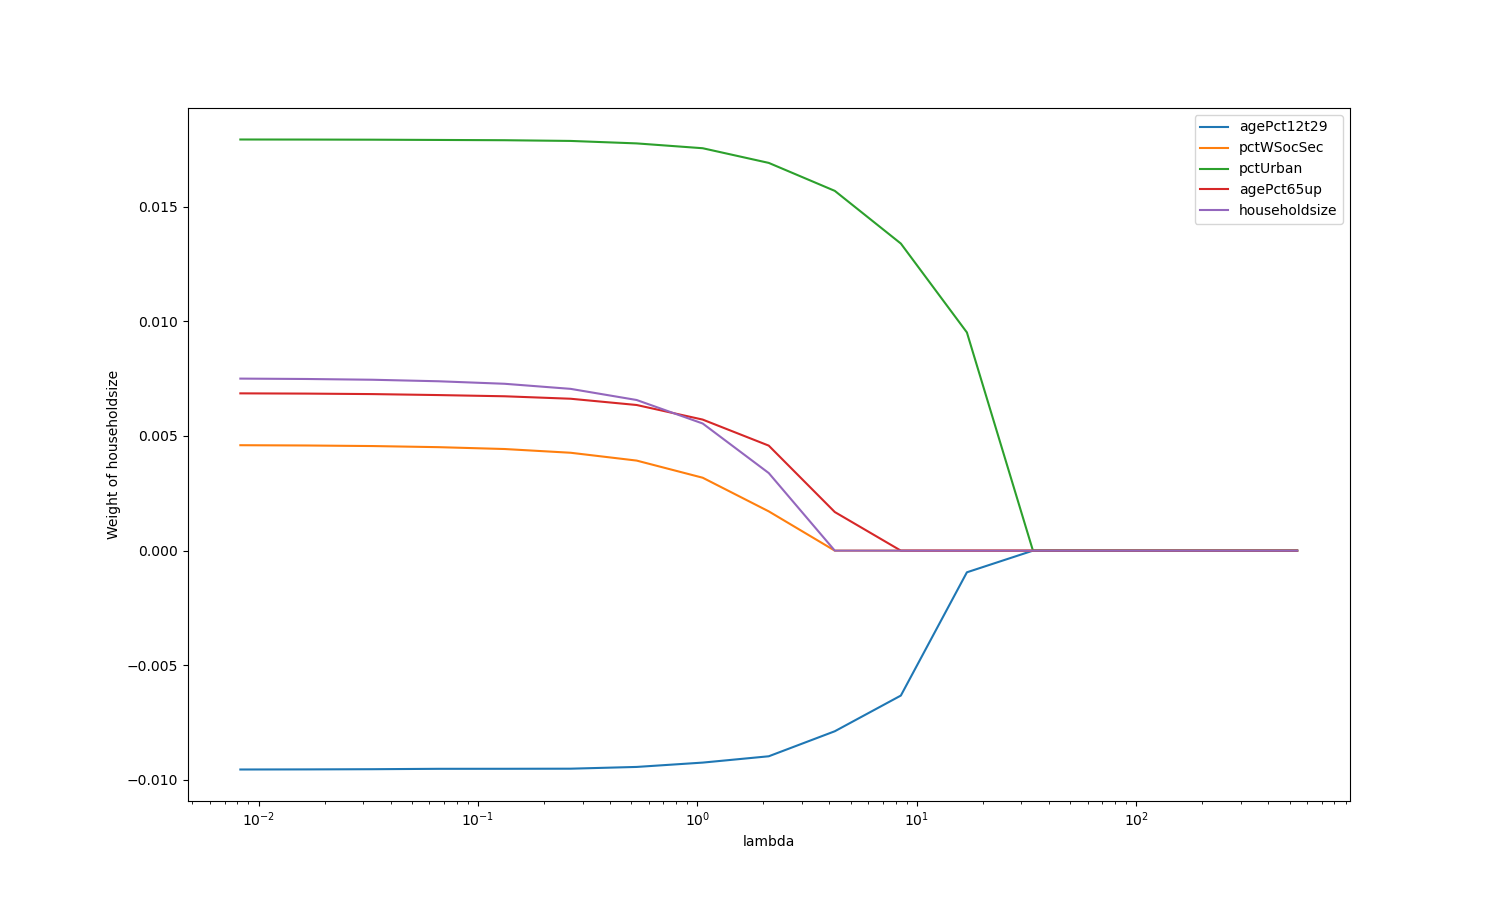
\includegraphics[width=\textwidth]{features_weight.png}
            \caption{Regularization paths for the coefficients of the variables}
        \end{figure}

        \item Here is the MSE on the training and test data:
        \begin{figure}[H]
            \centering
            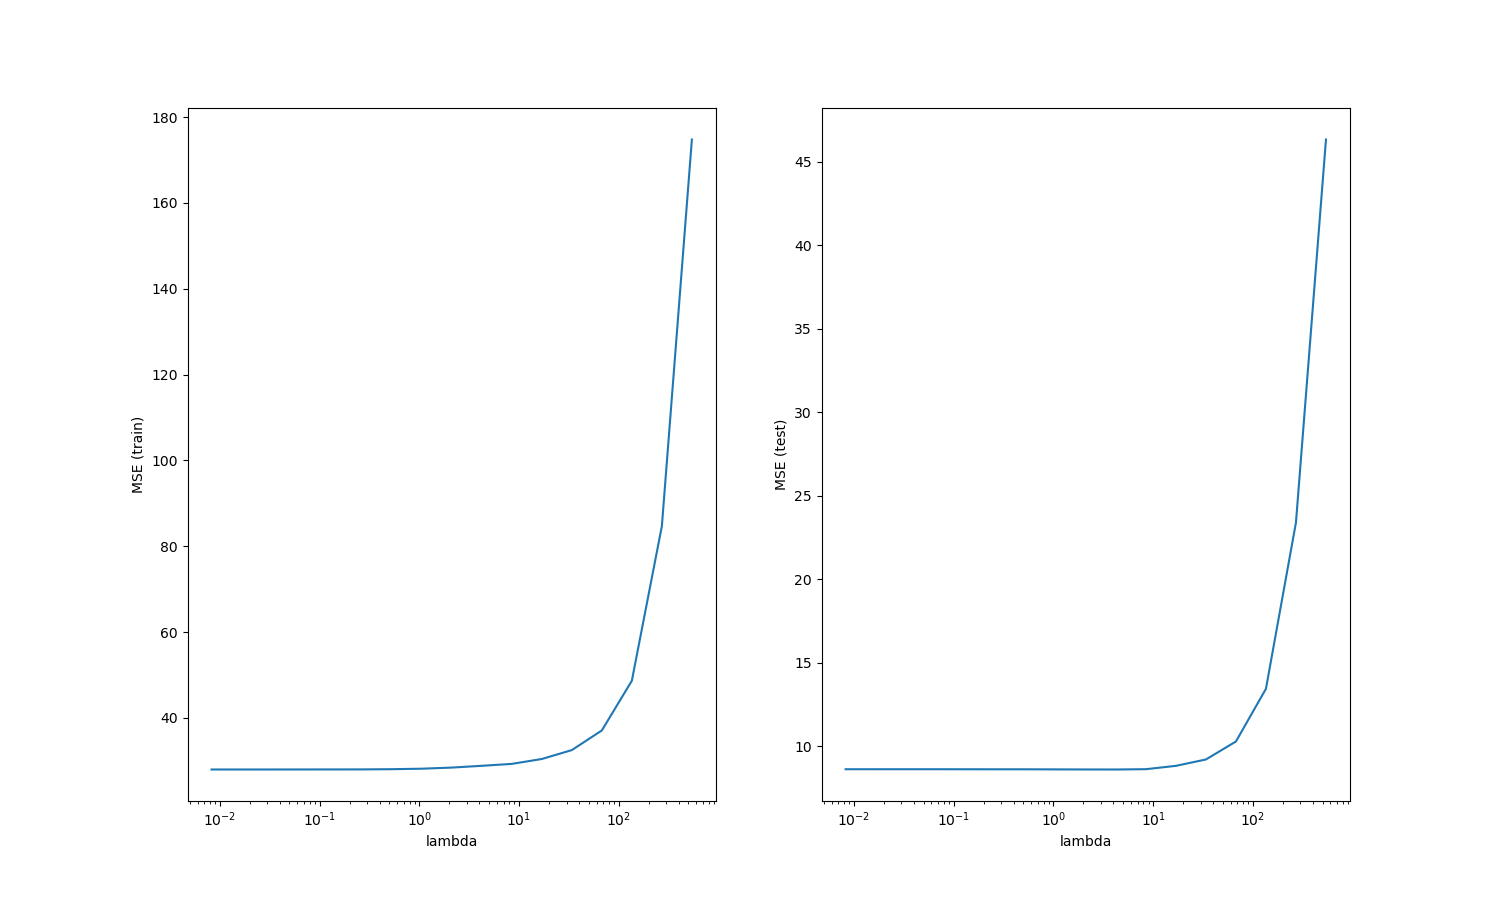
\includegraphics[width=0.8\textwidth]{MSE_crime.png}
            \caption{MSE on the training and test data}
        \end{figure}

        \item The most positive feature was PctIlleg and the most negative was PctKids2Par. I briefly mentioned this above when I was discussing the ethics, but this means that, under this model, the percentage of kids born to unmarried parents has the biggest correlation with violent crime, and the percentage of kids with 2 parents has the least correlation with violent crime.
        
        \item This is a correlation $\neq$ causation mistake. Fire trucks are often seen near burning buildings because they help clear fire. Fire trucks are extremely correlated with fire but instead of starting fires they put them out. Similarly, the agePct65up variable is not causing the crime, but instead could be a result of lower crime, such as less violent crime means less people are victims of murder, so more people will live longer, thus agePct65up goes up. In this manner agePct65up is correlated with less violent crime but is not the cause. 
    \end{enumerate}

    \subsection*{A7.}
    \begin{enumerate}[label=\alph*.]
        \item Notice that
        \begin{align*}
            \dv{x} \log(1+e^{-x}) = \frac{-e^{-x}}{1+e^{-x}} = \frac{1}{1+e^{-x}}-1
        \end{align*}
        We recall the chain rule: if $f: \R \to \R$, $g: \R^n \to \R$ are differentiable, then $\nabla_x (f \circ g)(x) = f'(g(x)) \nabla_x g(x)$. Taking $f(x) = \log(1+e^{-x})$ and $g(x) = y_i(b+x_i^Tw)$, we get that
        \begin{align*}
            \nabla_w \log(1+\exp(-y_i(b+x_i^Tw))) = \nabla_w f(g(x)) = \qty(\frac{1}{1+e^{-y_i(b+x_i^Tw)}}-1) y_ix_i = (\mu_i(w,b) - 1)y_ix_i
        \end{align*}
        Because $\nabla_w y_i(b+x_i^Tw) = \nabla_w y_ix_i^Tw = y_ix_i$. Similarly, 
        \begin{align*}
            \pdv{b} f(g(x)) = \qty(\frac{1}{1+e^{-y_i(b+x_i^Tw)}}-1) y_i = (\mu_i(w,b)-1)y_i
        \end{align*}
        Since $\nabla_w \lambda w^Tw = \lambda 2w$, we have that
        \begin{align*}
            \nabla_w J(w,b) &= \frac1n\sum_{i=1}^n \qty(\mu_i(w,b)-1)y_ix_i + 2\lambda w \\
            \pdv{b} J(w,b) &= \frac1n\sum_{i=1}^n \qty(\mu_i(w,b)-1)y_i
        \end{align*}

        \item 
        \begin{enumerate}[label=(\roman*)]
            \item Here is the plot of $J(w,b)$ as a function of the iteration number:
            \begin{figure}[H]
                \centering
                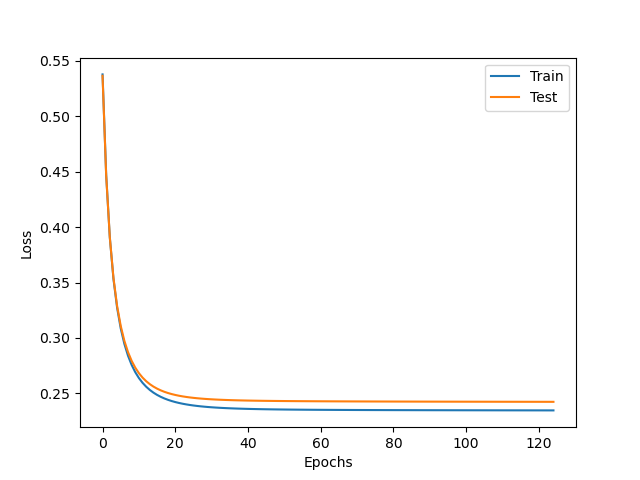
\includegraphics[width=0.6\textwidth]{grad_descent_loss.png}
                \caption{Loss as a function of the iteration number}
            \end{figure}

            \item Here is the plot of the miscalculation error as a function of the iteration number:
            \begin{figure}[H]
                \centering
                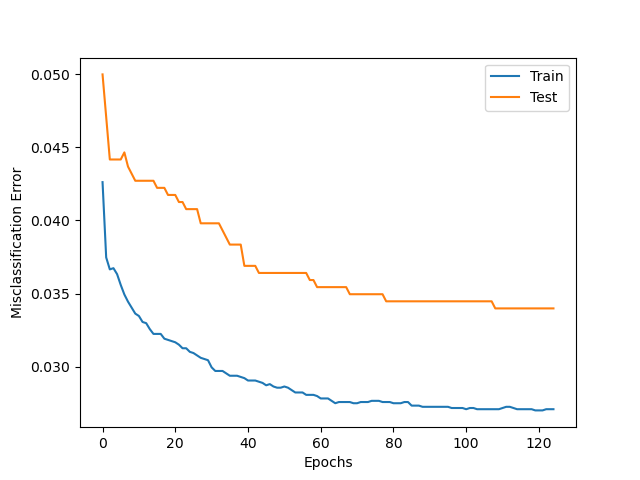
\includegraphics[width=0.6\textwidth]{grad_descent_misclass.png}
                \caption{Misclassification Error as a function of the iteration number}
            \end{figure}
        \end{enumerate}

        \item 
        \begin{enumerate}[label=(\roman*)]
            \item Loss for batch size 100:
            \begin{figure}[H]
                \centering
                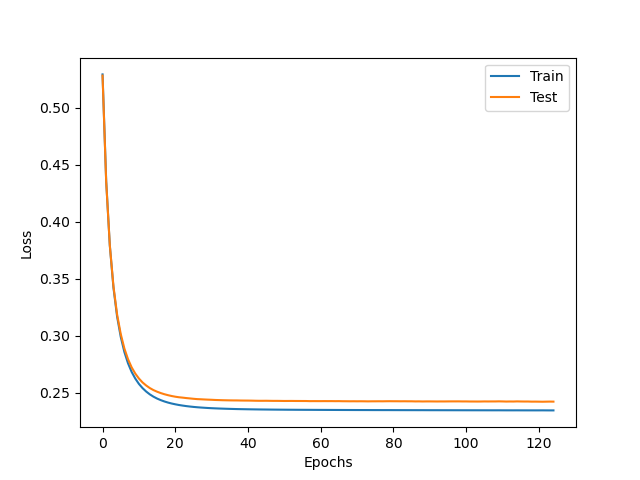
\includegraphics[width=0.6\textwidth]{SGD_batch_size_100_MSE.png}
                \caption{Loss as a function of the iteration number}
            \end{figure}

            \item Misclassification error for batch size 100:
            \begin{figure}[H]
                \centering
                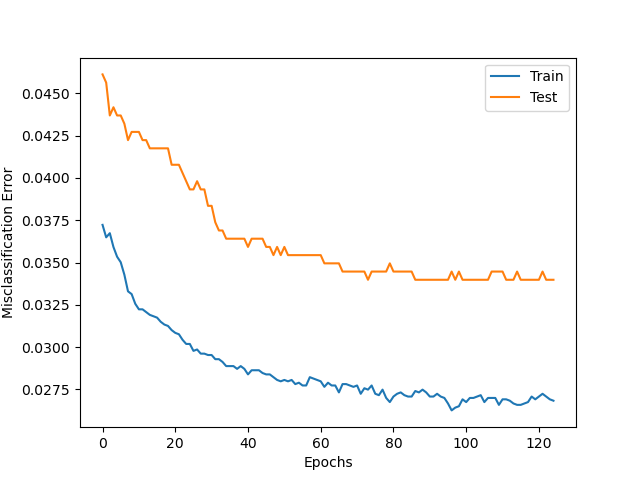
\includegraphics[width=0.6\textwidth]{SGD_batch_size_100_misclass.png}
                \caption{Misclassification Error as a function of the iteration number}
            \end{figure}
        \end{enumerate}

        \item 
        \begin{enumerate}[label=(\roman*)]
            \item Loss for batch size 1:
            \begin{figure}[H]
                \centering
                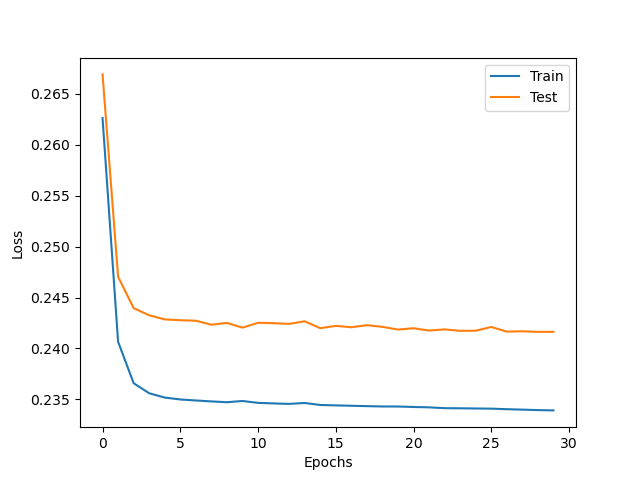
\includegraphics[width=0.6\textwidth]{batch_size_1_MSE.png}
                \caption{Loss as a function of the iteration number}
            \end{figure}

            \item Misclassification error for batch size 1:
            \begin{figure}[H]
                \centering
                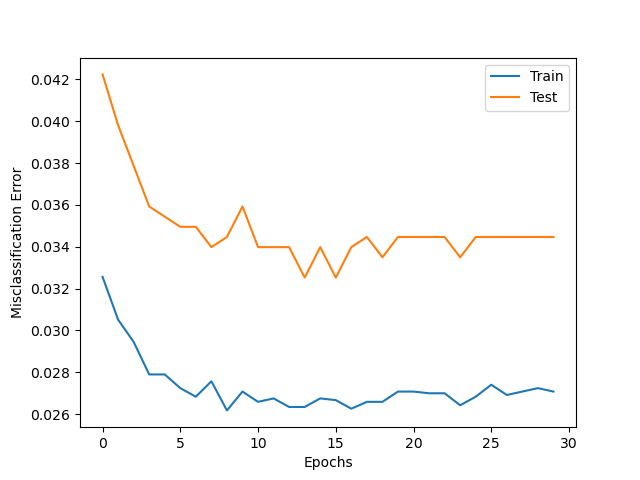
\includegraphics[width=0.6\textwidth]{batch_size_1_missclass.png}
                \caption{Misclassification Error as a function of the iteration number}
            \end{figure}
        \end{enumerate}
    \end{enumerate}

    \subsection*{A8.}
    \begin{enumerate}
        \item This homework took me around 12-15 hours to complete.
    \end{enumerate}
\end{document}